\documentclass[11pt,a4paper]{article}
\input{~/Documents/latex-config/math-preamble}
\newcommand{\problem}[1]{\textsc{#1}}
\title{DA4005 -- Homework set 2}
\author{David Sermoneta}
\date{\today}

\begin{document}
\maketitle
\begin{assignment}
 Let $L_1$ and $L_2$ be decidable languages over the same alphabet.
\begin{enumerate}[(a)]
 \item Prove that $L_1 \cup  L_2$ is decidable.
 \item Prove that $L_1\cap L_2$ is decidable.
 \item Suppose instead that $L_1$ and $L_2$ are only recognizable. Which of the two above statements remain true?
\end{enumerate}
\begin{proof}[Proof of (a)]
 If $T_1$ and $T_2$ are turing machines that decide $L_1$ and $L_2$ respectively, then let $T$ be the turing machine that given any input first is equivalent to $T_1$. Since $T_1$ halts on all inputs, we can model $T$ to go into an accepting state if $T_1$ accepts the input, and if not (i.e. $T_1$ rejects, which must happen since $T_1$ decides $L_1$, not just recognizes it), then $T$ feeds the input to $T_2$ and runs it anew. Now if $T_2$ accepts, $T$ accepts the input, and if $T_2$ rejects, $T$ now rejects the input. This means that $T$ recognizes $L_1\cup L_2$, and still halts on every input, so we are done.
\end{proof}

\begin{proof}[Proof of (b)]
 Let $T_1$ and $T_2$ be as before, then construct $T$ similarly to in the earlier proof, except $T$ only accepts the input only if it is both accepted by $T_1$ and $T_2$. In any other case (i.e. if $T_1$ or $T_2$ reject) $T$ rejects the input. Then $T$ by design halts again on every input, and so we are done.
\end{proof}

\begin{proof}[Proof of (c)]
 The statements are still true, but we have to be more careful about how we construct $T$. For $L_1 \cup L_2$, let $T_1$ and $T_2$ be as above, then we can design $T$ to run both $T_1$ and $T_2$ in parallel. We can think of this as running the same input for $T_1$ and $T_2$ on separate tapes, and for each operation on one tape, we switch tape. This means that if either $T_1$ or $T_2$ eventually accepts the input, $T$ enters an accepting state, and otherwise it keeps going (potentially for all eternity).

For the intersection $L_1\cap L_2$, the same machine $T$ works, except now it needs to accept only if both $T_1$  and $T_2$ accept the input. 
\end{proof}
\end{assignment}

\begin{assignment}
 Assume $A \leq_{p} B$.
\begin{enumerate}[(a)]
 \item Prove that if $B \in \mathcal{P}$, then $A \in  \mathcal{P}$.
 \item Prove that if $A$ is $\mathcal{NP}$-hard, then $B $ is $\mathcal{NP}$-hard.
 \item Explain why the direction of the reduction matters. Give a short example of an incorrect conclusion one might draw by reversing the arrow.
\end{enumerate}
\begin{proof}[Proof of (a)]
 If $A \leq_{p} B$ and $B \in \mathcal{P}$, then every instance of type $A$ can be rewritten in polynomial time into an instance of type $B$, and we can solve this translated instance in polynomial time.  Doing the translation, and then the solving the translated instance in polynomial time still results in a polynomial time solution, so we are done.
\end{proof}

\begin{proof}[Proof of (b)]
If $A$ is $\mathcal{NP}$-hard, it means that for any problem $C \in \mathcal{NP}$, 
$C \leq_{p} A$. But that means that $C \leq_{p} B$, since reduction in polynomial time is a transitive relation (two polynomial time algorithms is still a polynomial time algorithm). 
\end{proof}

\begin{proof}[Proof of (c)]
Really vague question IDK. If $B$ is $\mathcal{NP}$-hard, that alone says nothing about $A$, and if $A \in  \mathcal{P}$ that alone says nothing about $B$, I'm not sure what to come with here. 
\end{proof}
\end{assignment}

\begin{assignment}
 Define \problem{Two-satisfying-assignments} as follows. The input is a Boolean formula $\varphi$. The question is whether $\varphi$ has at least two distinct satisfying assignments.
\begin{enumerate}[(a)]
 \item Prove that \problem{Two-satisfying-assignments} is in $\mathcal{NP}$.
 \item Prove that it is $\mathcal{NP}$-hard by giving a polynomial-time reduction from \problem{SAT}.
 \item Explain why the two satisfying assignments in your construction are guaranteed to be distinct.
\end{enumerate}
\begin{proof}[Proof of (a)]
 It's in $\mathcal{NP}$ because a certificate is just a pair of distinct assignments of the free variables of $\varphi$, and checking whether or not they are valid is asymptotically equivalent  to checking whether or not one of them are, which is just a repeated verification of an instance of $\problem{Sat}$, which is already in $\mathcal{NP}$.
\end{proof}

\begin{proof}[Proof of (b) and (c)]
 So an instance of $\problem{Sat}$ is just a Boolean formula \[
 \varphi(x) = C_1 (x)\land \ldots \land C_{n}(x), 
\]
  where $x = (x_1,\ldots,x_{k}) $, $C_{i}(x_1,\ldots,x_{k}) = (x_{i_1} \lor \ldots \lor x_{i_{k}})$, and $x_{i_{j}} \in \{ x_1, \neg x_1 \ldots,x_{k}, \neg x_{k}\}$.
Then an assignment $e = (a_1,a_2,\ldots,a_{k})$ (where each $a_{i}$ is in $\{0,1\}$) satisfies $\varphi$ if $\varphi(e)$ is true.
Let \[
\psi(x_1,\ldots,x_{k}, \varepsilon) = \varphi(x_1,\ldots,x_{k}.
 \] Then we can treat $\psi$ as an instance of $\problem{Two-satisfying-assignments}$ that is our reduction, since showing $\psi$ has at least two different assignments that satisfy it, will in particular show that $\varphi$ has one, since both $\varepsilon = 0$ and $1$ doesn't change the truth value of $\psi$. This construction based on $\varphi$ is obviously polynomial, and so we are done.
\end{proof}
\end{assignment}

\begin{assignment}
 Recall that for a graph $G$, its \emph{chromatic polynomial $p_G(t)$} is the polynomial with the property that $p_G(j)$
gives the number of proper colorings of $G$ using at most $j$ colors.
\begin{enumerate}[(a)]
\item Prove that the chromatic polynomial of a graph with $n$ vertices has degree $n$.
\item Prove the chromatic polynomial of any tree with $n$ vertices is $t(t-1)^{n-1}$.
\item Show that if we can compute $p_G(t)$ for general graphs in polynomial time, then $\mathcal{P} = \mathcal{NP}$.
\end{enumerate}
\begin{proof}[Proof of (a)]
 For the complete graph on $n$ vertices, we have that the number of proper
colorings using at most $k \geq n$ colors is $\binom{n}{k} n!$. The reason for
this is that since all vertices are adjacent to all others, each coloring must
use $n$ distinct colors, and there are $\binom{n}{k}$ to choose from. For each
choice of $n$ colors, there are $n!$ distinct colorings of the graph and so by
multiplication principle we get the stated amount of colorings. 
Writing this out, we get a polynomial in $k$ of degree $n$, since this is just \[
p_{K_{n}}(k)= \frac{k!}{(k-n)!} = k(k-1)\ldots(k-n+2)(k-n+1),
\] and these correspond to the $n$ roots of $p_{K_{n}}$.
 For the complement of the complete graph, i.e. the graph on $n$ vertices with no edges,
the number of colorings is $k^{n}$, since we can choose any color $n$ times.
Now any other graph $G$ with $n$ vertices will have colorings bounded by these
two numbers. That is, we have \[ \binom{n}{k}n! \leq p_{G}(k) \leq k^{n}, \quad
k  \geq n.
 \] Since $p_{G}(k)$ is a polynomial bounded by two polynomials of degree $n$, asymptotically $p_{G}$ must also be a degree $n$ polynomial ($p_{G}(k) \in \Theta(k^{n})$).
\end{proof}

\begin{proof}[Proof of (b)]
 Let $T$ be a tree with $n$ vertices. We want to color it with at most $k$ colors. 
We start off by picking an arbitrary vertex $v$, this can be colored in $k$ different ways. Since a tree is acyclic, any adjacent vertex to $v$ will have $k-1$ possible choices, since these won't be adjacent to each other. Furthermore, any adjacent vertices to these will also have $k-1$ possible choices, since they cannot be connected to any other adjacent vertices, and so on. So the number of colorings is given by \[
k(k-1) ^{n-1}.
\] This means we are done, since this agrees with $p_{T}(k)$ for any $k$, and two 
polynomials cannot agree on an infinite set without being the same.
\end{proof}
\begin{proof}[Proof of (c)]
Well if we could, then it would be possible in polynomial time to compute whether or not a graph $G$ is 3-colorable. But the latter is $\mathcal{NP}$-complete, so we have that an $\mathcal{NP}$-complete problem is in $P$, i.e., $\mathcal{P} = \mathcal{NP}$.
\end{proof}

\end{assignment}

\begin{assignment}
Consider the directed weighted graph
\[
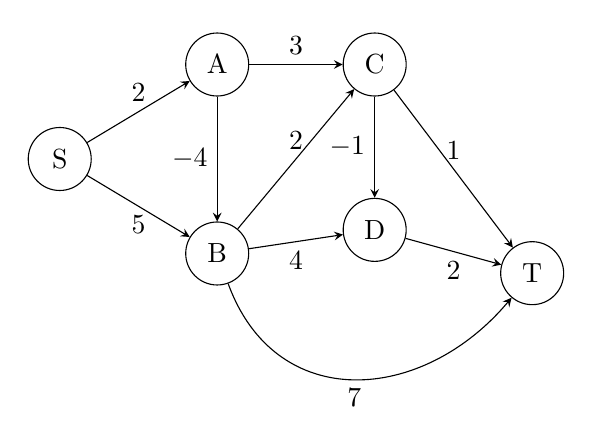
\begin{tikzpicture}[scale=1.0, >=stealth, vertex/.style={draw,circle,minimum size=8mm,inner sep=0pt}]
\node[vertex] (s) at (0,0) {$\mathrm{S}$};
\node[vertex] (a) at (2,1.2) {$\mathrm{A}$};
\node[vertex] (b) at (2,-1.2) {$\mathrm{B}$};
\node[vertex] (c) at (4,1.2) {$\mathrm{C}$};
\node[vertex] (d) at (4,-0.9) {$\mathrm{D}$};
\node[vertex] (t) at (6,-1.45) {$\mathrm{T}$};
\draw[->] (s) -- (a) node[midway,above] {$2$};
\draw[->] (s) -- (b) node[midway,below] {$5$};
\draw[->] (a) -- (b) node[midway,left] {$-4$};
\draw[->] (a) -- (c) node[midway,above] {$3$};
\draw[->] (b) -- (c) node[midway,above] {$2$};
\draw[->] (b) -- (d) node[midway,below] {$4$};
\draw[->] (c) -- (d) node[midway,left] {$-1$};
\draw[->] (c) -- (t) node[midway,above] {$1$};
\draw[->] (d) -- (t) node[midway,below] {$2$};
\draw[->] (b) to[out=-70,in=-130,looseness=1.25] node[midway,below] {$7$} (t);
\end{tikzpicture}
\]
In every pass, relax the edges in the order
$\mathrm{SA},\mathrm{SB},\mathrm{AB},\mathrm{AC},\mathrm{BC},
\mathrm{BD},\mathrm{CD},\mathrm{CT},\mathrm{DT},\mathrm{BT}$.
\begin{enumerate}[(a)]
\item Run Bellman--Ford from source $\mathrm{S}$. Show the distance estimates after each full pass over the edges.
\item Give the final shortest path tree.
\item Explain why Dijkstra's algorithm is not justified on this input, even if it might accidentally return correct distances for some edge orders.
\end{enumerate}
\begin{proof}[Solution of (a) and (b)]
 We actually only need to give one pass, since we get the shortest distances after just going through the edges once. This is because the edges are relaxed in the order that makes the smallest distance prioritized after $AB$, so each time we have to compare with an earlier relaxation, the distance is always larger than the distance given before. As stated, the only vertex not following this is $B$ that is first assigned distance $5$, to then afterwards be updated to $-2$ since $AB$ is relaxed after $SB$.
So here is the graph with updated distances after the first pass over the edges, as well as the last. The nodes drawn in red showcase also the shortest path (although getting to $T$ via $C$ is equivalent to going via $D$.)
\[
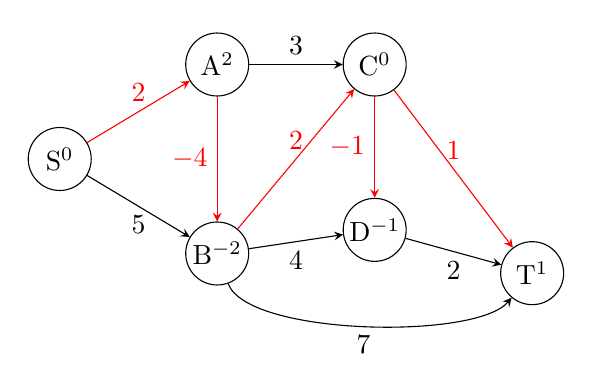
\begin{tikzpicture}[scale=1.0, >=stealth, vertex/.style={draw,circle,minimum size=8mm,inner sep=0pt}]
\node[vertex] (s) at (0,0) {$\mathrm{S}^{0}$};
\node[vertex] (a) at (2,1.2) {$\mathrm{A}^{2}$};
\node[vertex] (b) at (2,-1.2) {$\mathrm{B}^{-2}$};
\node[vertex] (c) at (4,1.2) {$\mathrm{C}^{0}$};
\node[vertex] (d) at (4,-0.9) {$\mathrm{D}^{-1}$};
\node[vertex] (t) at (6,-1.45) {$\mathrm{T}^{1}$};
\draw[->, red] (s) -- (a) node[midway,above] {$2$};
\draw[->] (s) -- (b) node[midway,below] {$5$};
\draw[->, red] (a) -- (b) node[midway,left] {$-4$};
\draw[->] (a) -- (c) node[midway,above] {$3$};
\draw[->, red] (b) -- (c) node[midway,above] {$2$};
\draw[->] (b) -- (d) node[midway,below] {$4$};
\draw[->, red] (c) -- (d) node[midway,left] {$-1$};
\draw[->, red] (c) -- (t) node[midway,above] {$1$};
\draw[->] (d) -- (t) node[midway,below] {$2$};
\draw[->] (b) to[out=-70,in=-130,looseness=0.5] node[midway,below] {$7$} (t);
\end{tikzpicture}
\]
\end{proof}
\begin{proof}[Solution of (c)]
I think it does accept the whole input, but let's say that the weight on $(S,B)$ were $1$, then $B$ would be the nearest vertex from $S$, and that would instantly become the shortest path, because when we then check the neighbors of $A$, we don't consider the edge $(A,B)$, since $B$ is already visited, even though it gives a shorter distance. (MAYBE this kind of argument could be made on this particular graph without any modifications, but I wasn't able to find it so this is my explanation). 
\end{proof}
\end{assignment}

\begin{assignment}
Two friends leave a party at vertex $s$ of a connected undirected graph
$G=(V,E)$.  Their homes are at distinct vertices $a$ and $b$.  Every road
$e$ has a nonnegative length $w(e)$.  They may choose a vertex $v$, walk
together along one route from $s$ to $v$, and then each walk alone from $v$
to their home.

Walking in company makes a road feel $50\%$ shorter.
A road of length $w$ traversed by one friend alone contributes $w$ to the total inconvenience, whereas the
same road traversed together contributes only $w$ rather than $2w$. 
Their goal is to minimize their total inconvenience.
\begin{enumerate}[(a)]
\item For a fixed separation vertex $v$, express the least possible total
inconvenience using shortest-path distances among $s,v,a,b$.  Justify your
expression.
\item Give a polynomial-time algorithm that finds the optimal $v$ and
reconstructs the three routes.
Argue why the algorithm is correct and runs in polynomial time.

\item Give a small example in which an optimal solution makes at least one
friend take a route strictly longer than their own shortest route home, in
exchange for walking farther together.
\end{enumerate}
\end{assignment}
\end{document}
